\documentclass{article}

% if you need to pass options to natbib, use, e.g.:
% \PassOptionsToPackage{numbers, compress}{natbib}
% before loading nips_2016
%
% to avoid loading the natbib package, add option nonatbib:
% \usepackage[nonatbib]{nips_2016}

% \usepackage[final]{nips_2016}

% to compile a camera-ready version, add the [final] option, e.g.:
\usepackage[final]{nips_2016}

\usepackage[utf8]{inputenc} % allow utf-8 input
\usepackage[T1]{fontenc}    % use 8-bit T1 fonts
\usepackage{hyperref}       % hyperlinks
\usepackage{url}            % simple URL typesetting
\usepackage{booktabs}       % professional-quality tables
\usepackage{amsfonts}       % blackboard math symbols
\usepackage{nicefrac}       % compact symbols for 1/2, etc.
\usepackage{microtype}      % microtypography

\usepackage{graphicx}
\graphicspath{ {tu/} }

\usepackage{caption}
\usepackage{subcaption}

\title{On-hands Study of Tree-based Methods}

% The \author macro works with any number of authors. There are two
% commands used to separate the names and addresses of multiple
% authors: \And and \AND.
%
% Using \And between authors leaves it to LaTeX to determine where to
% break the lines. Using \AND forces a line break at that point. So,
% if LaTeX puts 3 of 4 authors names on the first line, and the last
% on the second line, try using \AND instead of \And before the third
% author name.

\author{
  Chenyang~Dong\\
  Department of Mathematics\\
  \texttt{cdongac@connect.ust.hk} \\
  \And
  Tsz Cheung~Lo\\
   Department of Computer Science\\
  \texttt{tcloaa@connect.ust.hk} \\
  \And
  Jiacheng~Xia\\
   Department of Computer Science\\
  \texttt{jxiaab@connect.ust.hk} \\
  %% examples of more authors
  %% \And
  %% Coauthor \\
  %% Affiliation \\
  %% Address \\
  %% \texttt{email} \\
  %% \AND
  %% Coauthor \\
  %% Affiliation \\
  %% Address \\
  %% \texttt{email} \\
  %% \And
  %% Coauthor \\
  %% Affiliation \\
  %% Address \\
  %% \texttt{email} \\
  %% \And
  %% Coauthor \\
  %% Affiliation \\
  %% Address \\
  %% \texttt{email} \\
}

\begin{document}
% \nipsfinalcopy is no longer used

\maketitle

\begin{abstract}
Intentionally left blank
\end{abstract}

\section{Introduction}

For the past few lectures we have gone through more methods for doing regression and classification analysis. Among them we decided to go for a study on tree-based methods for the second mini-project. We use tree-based methods both on the America Crime Dataset and the In-class Kaggle competitions, and we find that tree-based methods are straightforward to implement and can give satisfying performance. In this report we present the results for both tests.

The rest of the report is organized as following: Section \ref{crime-Lasso} describes the crime dataset and our previous results in project 1 using Lasso, and make comparisons between Lasso and tree-based methods. Section \ref{combodrug} describes how we used tree-based methods for combinatoric-valued drug data, their results and model comparisons. Section \ref{drug2} presents our results on the in-class Kaggle Competition: Binary DrugSensitivity2 Data. In the end there is a concluding part summarizing our findings and comments on tree-based methods.

\section{Crime dataset and previous results}
\label{crime-Lasso}
In this section we present the tree based analysis for the crime data. Firstly we describe of the results using regression tree analysis and further optimized by bagging and boosting. In the end the results were compared with Lasso which we used on same dataset for project 1.

\subsection{The American Crime dataset}
\label{crime_data}
This dataset contains the statistics of crime rate of 7 types in American cities from 1970 to 1992. Besides the name and abbreviation attributes there are 23 features like city population size, number of police, income per capita etc. There are more than 1000 valid data with complete information in this form. Since the features are of different scales, we preprocessed the data by first centering it along the axis to the mean, and component-wise scaling to unit variance.
\subsection{previous results}
In the first mini-project, we used various methods to analyze the crime data, and we found that Lasso does best in terms of both prediction and feature selection. Since the seven kinds of crimes are analyzed seperately, we focus on the crime type "Larceny" and we observed that other crime types gave similar results. Lasso gave a test set mean-squared-error (MSE) for around 0.06. We would use this as a benchmark.

\subsection{Regression tree analysis}
\label{crime_reg_tree}
We first did a regression tree analysis from the tree analysis. We randomly split 90\% of the data as training set and rest as testing set and got a mean-squared error as 0.1157. As we can see in the graph, regression tree also did well in feature selection, picking out city population, age structure and police forces, which is consistent with our conclusion in project 1.
\begin{figure}[h]
  \centering
  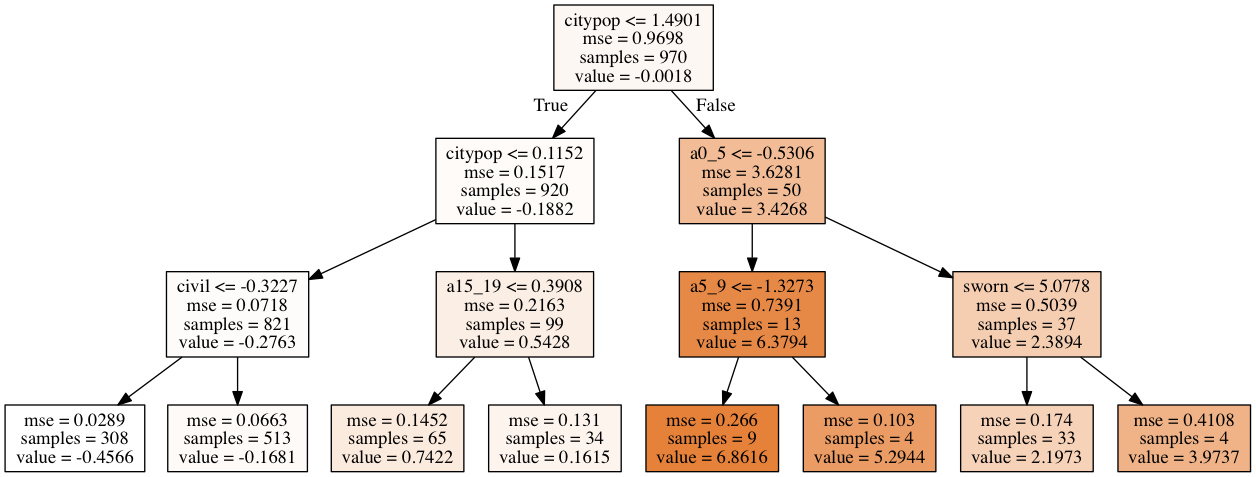
\includegraphics[width=10cm, height=4cm]{crime_treetu}
  \caption{Regression tree on crime data}
\end{figure}

\begin{figure}
\centering
\begin{minipage}{.5\textwidth}
  \centering
  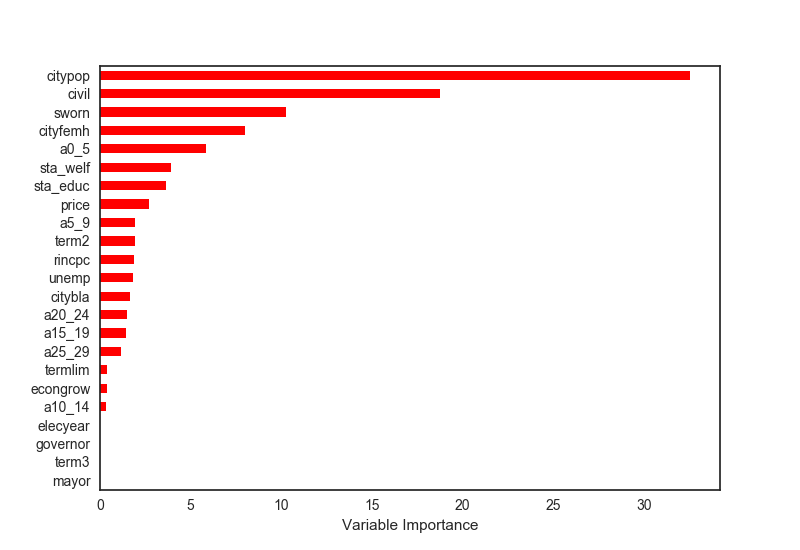
\includegraphics[width=.8\linewidth,height=4cm]{crime_boosttu}
  \captionof{figure}{Importance\\ from boosting}
  \label{fig:test1}
\end{minipage}%
\begin{minipage}{.5\textwidth}
  \centering
  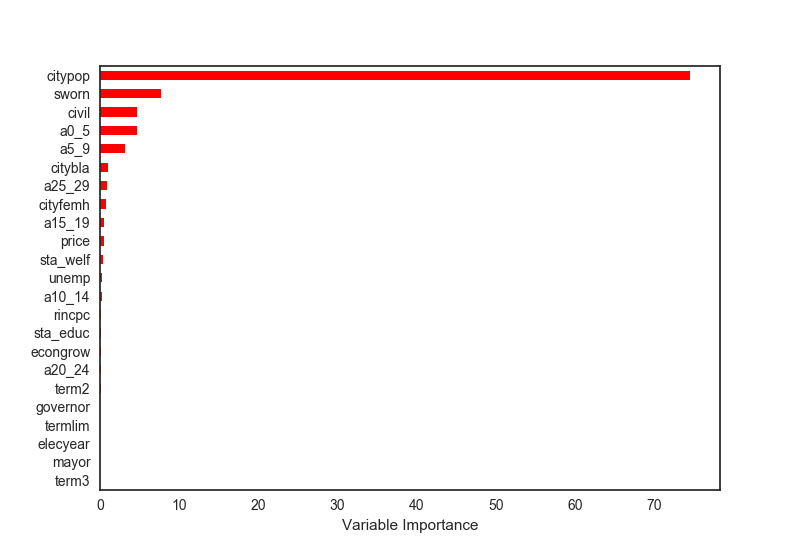
\includegraphics[width=.8\linewidth,height=4cm]{crime_randtu}
  \captionof{figure}{Importance\\ from random forest}
  \label{fig:test2}
\end{minipage}
\end{figure}


\subsection{Boosting and Random forest}
To optimize the results from the regression tree, we tried random forest and gradient boosting methods. We found that gradient boosting gives a testing error of 0.04 and random forest using all features further reduces the results to 0.02. To compare the reason we plot the variable importance which indicates the reduction in Gini index if we eliminate this variable, and as shown random forest gives a good indication that \textit{citypop} is the dominating feature. So in such kind of data where only one feature dominates, we can see that the Random Forest performs better.

\subsection{Remarks}
Despite tree-based methods generally perform better in the crime dataset, we can not yet conclude that tree-based methods would always perform better, since crime data is low dimension with only very few important features and they have different importance, and tree-based methods can intuitively perform well in such cases. It remains to see the results in the in-Kaggle competition, whose data has some different features.

\section{Analysis of Combinatoric Drug20 using Tree-based methods}
\label{combodrug}

\section{Results of Binary DrugSensitivity2}
\label{drug2}

\section{Conclusion}
\label{con}

\subsubsection*{Acknowledgments}
\section*{References}
\small
[1] Alexander, J.A.\ \& Mozer, M.C.\ (1995) Template-based algorithms
for connectionist rule extraction. In G.\ Tesauro, D.S.\ Touretzky and
T.K.\ Leen (eds.), {\it Advances in Neural Information Processing
  Systems 7}, pp.\ 609--616. Cambridge, MA: MIT Press.
\end{document}
